% Options for packages loaded elsewhere
\PassOptionsToPackage{unicode}{hyperref}
\PassOptionsToPackage{hyphens}{url}
%
\documentclass[
]{book}
\usepackage{amsmath,amssymb}
\usepackage{lmodern}
\usepackage{iftex}
\ifPDFTeX
  \usepackage[T1]{fontenc}
  \usepackage[utf8]{inputenc}
  \usepackage{textcomp} % provide euro and other symbols
\else % if luatex or xetex
  \usepackage{unicode-math}
  \defaultfontfeatures{Scale=MatchLowercase}
  \defaultfontfeatures[\rmfamily]{Ligatures=TeX,Scale=1}
\fi
% Use upquote if available, for straight quotes in verbatim environments
\IfFileExists{upquote.sty}{\usepackage{upquote}}{}
\IfFileExists{microtype.sty}{% use microtype if available
  \usepackage[]{microtype}
  \UseMicrotypeSet[protrusion]{basicmath} % disable protrusion for tt fonts
}{}
\makeatletter
\@ifundefined{KOMAClassName}{% if non-KOMA class
  \IfFileExists{parskip.sty}{%
    \usepackage{parskip}
  }{% else
    \setlength{\parindent}{0pt}
    \setlength{\parskip}{6pt plus 2pt minus 1pt}}
}{% if KOMA class
  \KOMAoptions{parskip=half}}
\makeatother
\usepackage{xcolor}
\IfFileExists{xurl.sty}{\usepackage{xurl}}{} % add URL line breaks if available
\IfFileExists{bookmark.sty}{\usepackage{bookmark}}{\usepackage{hyperref}}
\hypersetup{
  pdftitle={Supplementary Materials for Gene Co-expression Network Estimation for Spatial Transcriptomics},
  pdfauthor={Satwik Acharyya, Xiang Zhou, Veera Baladandayuthapani},
  hidelinks,
  pdfcreator={LaTeX via pandoc}}
\urlstyle{same} % disable monospaced font for URLs
\usepackage{color}
\usepackage{fancyvrb}
\newcommand{\VerbBar}{|}
\newcommand{\VERB}{\Verb[commandchars=\\\{\}]}
\DefineVerbatimEnvironment{Highlighting}{Verbatim}{commandchars=\\\{\}}
% Add ',fontsize=\small' for more characters per line
\usepackage{framed}
\definecolor{shadecolor}{RGB}{248,248,248}
\newenvironment{Shaded}{\begin{snugshade}}{\end{snugshade}}
\newcommand{\AlertTok}[1]{\textcolor[rgb]{0.94,0.16,0.16}{#1}}
\newcommand{\AnnotationTok}[1]{\textcolor[rgb]{0.56,0.35,0.01}{\textbf{\textit{#1}}}}
\newcommand{\AttributeTok}[1]{\textcolor[rgb]{0.77,0.63,0.00}{#1}}
\newcommand{\BaseNTok}[1]{\textcolor[rgb]{0.00,0.00,0.81}{#1}}
\newcommand{\BuiltInTok}[1]{#1}
\newcommand{\CharTok}[1]{\textcolor[rgb]{0.31,0.60,0.02}{#1}}
\newcommand{\CommentTok}[1]{\textcolor[rgb]{0.56,0.35,0.01}{\textit{#1}}}
\newcommand{\CommentVarTok}[1]{\textcolor[rgb]{0.56,0.35,0.01}{\textbf{\textit{#1}}}}
\newcommand{\ConstantTok}[1]{\textcolor[rgb]{0.00,0.00,0.00}{#1}}
\newcommand{\ControlFlowTok}[1]{\textcolor[rgb]{0.13,0.29,0.53}{\textbf{#1}}}
\newcommand{\DataTypeTok}[1]{\textcolor[rgb]{0.13,0.29,0.53}{#1}}
\newcommand{\DecValTok}[1]{\textcolor[rgb]{0.00,0.00,0.81}{#1}}
\newcommand{\DocumentationTok}[1]{\textcolor[rgb]{0.56,0.35,0.01}{\textbf{\textit{#1}}}}
\newcommand{\ErrorTok}[1]{\textcolor[rgb]{0.64,0.00,0.00}{\textbf{#1}}}
\newcommand{\ExtensionTok}[1]{#1}
\newcommand{\FloatTok}[1]{\textcolor[rgb]{0.00,0.00,0.81}{#1}}
\newcommand{\FunctionTok}[1]{\textcolor[rgb]{0.00,0.00,0.00}{#1}}
\newcommand{\ImportTok}[1]{#1}
\newcommand{\InformationTok}[1]{\textcolor[rgb]{0.56,0.35,0.01}{\textbf{\textit{#1}}}}
\newcommand{\KeywordTok}[1]{\textcolor[rgb]{0.13,0.29,0.53}{\textbf{#1}}}
\newcommand{\NormalTok}[1]{#1}
\newcommand{\OperatorTok}[1]{\textcolor[rgb]{0.81,0.36,0.00}{\textbf{#1}}}
\newcommand{\OtherTok}[1]{\textcolor[rgb]{0.56,0.35,0.01}{#1}}
\newcommand{\PreprocessorTok}[1]{\textcolor[rgb]{0.56,0.35,0.01}{\textit{#1}}}
\newcommand{\RegionMarkerTok}[1]{#1}
\newcommand{\SpecialCharTok}[1]{\textcolor[rgb]{0.00,0.00,0.00}{#1}}
\newcommand{\SpecialStringTok}[1]{\textcolor[rgb]{0.31,0.60,0.02}{#1}}
\newcommand{\StringTok}[1]{\textcolor[rgb]{0.31,0.60,0.02}{#1}}
\newcommand{\VariableTok}[1]{\textcolor[rgb]{0.00,0.00,0.00}{#1}}
\newcommand{\VerbatimStringTok}[1]{\textcolor[rgb]{0.31,0.60,0.02}{#1}}
\newcommand{\WarningTok}[1]{\textcolor[rgb]{0.56,0.35,0.01}{\textbf{\textit{#1}}}}
\usepackage{longtable,booktabs,array}
\usepackage{calc} % for calculating minipage widths
% Correct order of tables after \paragraph or \subparagraph
\usepackage{etoolbox}
\makeatletter
\patchcmd\longtable{\par}{\if@noskipsec\mbox{}\fi\par}{}{}
\makeatother
% Allow footnotes in longtable head/foot
\IfFileExists{footnotehyper.sty}{\usepackage{footnotehyper}}{\usepackage{footnote}}
\makesavenoteenv{longtable}
\usepackage{graphicx}
\makeatletter
\def\maxwidth{\ifdim\Gin@nat@width>\linewidth\linewidth\else\Gin@nat@width\fi}
\def\maxheight{\ifdim\Gin@nat@height>\textheight\textheight\else\Gin@nat@height\fi}
\makeatother
% Scale images if necessary, so that they will not overflow the page
% margins by default, and it is still possible to overwrite the defaults
% using explicit options in \includegraphics[width, height, ...]{}
\setkeys{Gin}{width=\maxwidth,height=\maxheight,keepaspectratio}
% Set default figure placement to htbp
\makeatletter
\def\fps@figure{htbp}
\makeatother
\setlength{\emergencystretch}{3em} % prevent overfull lines
\providecommand{\tightlist}{%
  \setlength{\itemsep}{0pt}\setlength{\parskip}{0pt}}
\setcounter{secnumdepth}{5}
\usepackage{booktabs}
 \usepackage{amsmath, amsthm, amssymb, bbm, setspace,bigints}
\makeatletter
\def\thm@space@setup{%
  \thm@preskip=8pt plus 2pt minus 4pt
  \thm@postskip=\thm@preskip
}
\makeatother
\usepackage{booktabs}

\def\T{{ \mathrm{\scriptscriptstyle T} }}
\def\tr{{\rm tr\,}}
\ifLuaTeX
  \usepackage{selnolig}  % disable illegal ligatures
\fi
\usepackage[]{natbib}
\bibliographystyle{apalike}

\title{Supplementary Materials for Gene Co-expression Network Estimation for Spatial Transcriptomics}
\author{Satwik Acharyya, Xiang Zhou, Veera Baladandayuthapani}
\date{2022-05-19}

\begin{document}
\maketitle

{
\setcounter{tocdepth}{1}
\tableofcontents
}
\hypertarget{appendix-supplementary-materials}{%
\appendix}


\hypertarget{introduction}{%
\chapter*{Introduction}\label{introduction}}
\addcontentsline{toc}{chapter}{Introduction}

The spatial transcriptomics method depicts the positioning of a single cell on a spatially structured tissue. Knowledge about gene expressions and the spatial distribution of mRNA allows us to uncover cellular and subcellular heterogeneity in tissues, tumors, and immune cells. Spatial transcriptomics provides a unique opportunity to decipher both the cellular and subcellular architecture in both tissues and individual cells along with detection of gene co-expression patterns at both levels. These approaches are very insightful to study disease propagation in the field of embryology, oncology, and histology. The SpaceX method is a statistical tool to quantify spatially varying gene co-expression patterns in a tissue consists of different cell type based or sptailly contiguous clusters.

This is a supplementary file of the paper named SpaceX: Gene Co-expression Network Estimation in Spatial Transcriptomics. The sectional contents of the supplementary file is mentioned below.

\begin{enumerate}
\def\labelenumi{\arabic{enumi}.}
\tightlist
\item
  We start with a detailed description of the methodology in section \ref{method}.
\item
  In section \ref{simulation}, further details of simulation study have been discussed.
\item
  Eploratory analysis and more findings of real data analysis have been laid out in section \ref{realdata}.
\item
  Finally, we discuss the detailed steps for implementation of the SpaceX package in section \ref{ImplementSpaceX}.
\end{enumerate}

\hypertarget{method}{%
\chapter{Methodology}\label{method}}

In this section, we start with a brief discussion of the model and interpretations of each term of the model. Next, A detailed discussion of the estimation procedure for the SpaceX model in equation 1 in section 2 of the paper (also mentioned in equation \eqref{eq:Poi-mean-model-matrix-rev} ) is provided. Finally we discuss the methodological novelty of our SpaceX method.

\hypertarget{spacex-model}{%
\section{SpaceX model}\label{spacex-model}}

The gene expression is modeled with a Poisson distribution as
\begin{equation}
y^{c}_{g}({\bf s}_{i}) \sim \text{Poi}\{ M^{c}({\bf s}_{i}) \lambda^{c}_{g}({\bf s}_{i})\}.
\label{eq:SpaceX-supp}
\end{equation}
The interpretations of the notations in equation \eqref{eq:SpaceX-supp} remains same as mentioned in the section 2.2 of the paper. We denote \(\Lambda^{c}\) as a \(G \times N_{c}\) (\(N_{c}\) denotes size of the c-th cluster) matrix containing the rate parameters for all genes and c-th cluster.
Subsequently, we model the cluster specific and spatially dependent rate parameter \(\bf \Lambda^{c}\) with an additive log-linear equation, i.e.~
\begin{equation}
\text{log}({\bf \Lambda}^{c}) = {\bf B}^{c}{\bf X}^{c} + {\bf S}^{c} + {\bf \Phi F} + {\bf \Psi^{c} D^{c}} + {\boldsymbol{\mathcal{E}}}^{c}.
\label{eq:Poi-mean-model-matrix-rev}
\end{equation}

We clearly mention the shared and cluster-specific parameters and their interpretations table \ref{tab:sharedclusterelements}.

Parameters

Shared

Cluster-specific

Interpretations

\({\bf B}^{c}{\bf X}^{c}\)

\(\times\)

\(\checkmark\)

Covariate effect

\({\bf S}^{c}\)

\(\times\)

\(\checkmark\)

Spatial information

\({\bf \Phi F}\)

\(\checkmark\)

\(\times\)

Shared loadings and factors

\(\bf \Psi^{c} D^{c}\)

\(\times\)

\(\checkmark\)

Cluster loadings and factors

\(\boldsymbol{\mathcal{E}}^{c}\)

\(\times\)

\(\checkmark\)

Error matrix

\label{tab:sharedclusterelements} Shared and cluster-specific parameters along with their corresponding interpretations.

A full-scale MCMC will be computationally expensive on a complex hierarchical model. For computational advantage, we decompose the model into two parts (I) sPMM: spatial Poisson mixed model \citep{sun2018heritability} and (II) MSFA: Multi-study factor analysis model \citep{de2018bayesian}. We enable this model decomposition through a standard Gaussian random variable.

\hypertarget{poisson-mixed-model}{%
\section{Poisson Mixed Model}\label{poisson-mixed-model}}

We can break the SpaceX model \eqref{eq:Poi-mean-model-matrix-rev} and write the spatial Poisson mixed model as

\begin{align}
\begin{split}
& \text{log}({\boldsymbol \lambda}^{c}_{g}) = {{\bf X}^{c}}^{T} {\boldsymbol \beta}^{c}_{g} + {\bf s}^{c} + {\bf z}^{c}_{g}, \\
& {\boldsymbol \lambda}^{c}_{g} = ( \lambda^{c}_{1g}, \dots , \lambda^{c}_{N_{c}g} )^{T}, \\
&{\bf s}^{c} = ( s^{c}_{1}, \dots , s^{c}_{N_{c}} )^{T} \sim \text{MVN}(0, \sigma_{1}^{2}\Omega^{c}(s)), \\
&{\bf z}^{c}_{g} = (z^{1}_{1g}, \dots , z^{c}_{N_{c}g})^{T} \sim \text{MVN}(0, \sigma_{2}^{2} I_{N_{c} \times N_{c} }).
\end{split}
\label{eq:PMM-supp}
\end{align}

Here \(\Omega^{c}(s_{1}, s_{2}) = \text{exp} (- \mid \mid s_{1} - s_{2} \mid \mid^{2} / 2 \rho^{2}_{c} ),\) \(c = 1, \dots, C\). We estimate the length scale parameter of spatial kernel \(\rho_{c}\) based on the steps discussed in section 1 of supplementary information in \citet{sun2020statistical}. Here \(Z^{c}_{g}\) captures the cluster specific latent gene expressions and a multi-variate hierarchical modeling of \(Z^{c}_{g}(s_{i})\) will help us to identify the gene co-expression network.

\hypertarget{multi-study-factor-model-msfa}{%
\section{Multi-Study Factor Model (MSFA)}\label{multi-study-factor-model-msfa}}

The 2nd stage of the modeling framework is multi-study factor analysis \citep{de2018bayesian} which is provided as follows
\begin{align}
\begin{split}
& \hat{\bf z}^{c}_{i} = \boldsymbol \Phi {\bf f}_{i} + \boldsymbol \Psi^{c} {\bf d}^{c}_{i} + {\bf e}^{c}_{i}, \\
& {\bf f}_{i} \sim N_{K}(0, {\bf I}_{K}), \hspace{0.5cm} {\bf d}^{c}_{i} \sim N_{K_{c}}(0,{\bf I}_{K_{c}}),\\
& {\bf e}^{c}_{i} \sim N_{G}(0,\boldsymbol \Xi_{c}), \hspace{0.5cm} \boldsymbol \Xi_{c} = \text{diag}(\xi^{c}_{1}, \dots, \xi^{c}_{G} ).
\end{split}
\label{eq:MSFA-supp}
\end{align}
The marginal distribution of \(\hat{\bf z}^{c}_{i}\) is a multivariate normal distribution with mean \(0\) and covariance matrix \(\Sigma_{c}\) s.t.
\begin{align}
\Sigma_{c} = \Phi \Phi^{T} + \Psi^{c} {\Psi^{c}}^{T} + \Xi_{c} = \Sigma_{\Phi} + \Sigma_{\Psi^{c}} + \Xi_{c}
\label{eq:sigma-decomposition}
\end{align}
\(\Sigma_{\Phi} = \Phi \Phi^{T}\) and \(\Sigma_{\Psi^{c}} = \Psi^{c} {\Psi^{c}}^{T}\) are covariance of shared and cluster specific factors respectively. The decomposition of \(\Sigma_{c}\) in \eqref{eq:sigma-decomposition} is not a unique since we can set \(\Phi^{*} = \Phi Q\) and \({\Psi^{*}}^{c} = \Psi^{c} Q_{c}\) where \(Q\) and \(Q_{c}\) are square orthonormal matrices. This will also lead to the same decomposition \(\Sigma^{c} = \Phi^{*} {\Phi^{*}}^{T} + {\Psi^{*}}^{c} {{\Psi^{*}}^{c}}^{T} = \Phi \Phi^{T} + \Psi_{c} \Psi_{c}^{T}\). To overcome the indeterminacy through orthonormal matrices, the factor loading matrices are restricted to be lower triangular matrices \citep{geweke1996measuring, lopes2004bayesian}.

\hypertarget{multiplicative-gamma-shrinkage-prior}{%
\section{Multiplicative gamma shrinkage prior}\label{multiplicative-gamma-shrinkage-prior}}

We follow the same steps from \citet{de2018bayesian} and place multiplicative gamma shrinkage prior \citep{bhattacharya2011sparse} prior on the shared and cluster specific loading matrices i.e.~\(\Phi\) and \(\Psi_{c}\) \(c=1,\dots,C\). The shared and cluster specific latent factors (\(K\) and \(K_{c}\) respectively) are selected following methodology described in section 3.3 of \citet{de2018bayesian}. The multiplicative gamma prior on elements of shared covariance matrices are provided as follows
\begin{equation}
\begin{split}
& \phi_{gk} \mid \delta_{gk}, \eta_{k} \sim N(0, \delta_{gk}^{-1} \eta_{k}^{-1}), \hspace{0.5cm} g = 1, \dots , G, \hspace{0.25cm} k = 1, \dots, \infty, \\
& \delta_{gk} \sim \Gamma(\frac{\nu}{2}, \frac{\nu}{2}) \hspace{0.5cm}  \eta_{k} = \prod_{j=1}^{k} \zeta_{j} \hspace{0.5cm} \zeta_{1} \sim \Gamma(a_{1},1) \hspace{0.5cm}  \zeta_{j} \sim \Gamma(a_{2},1), \hspace{0.2cm} j \ge 2. 
\end{split}
\end{equation}
Here \(\delta_{gk}\) is the local shrinkage parameter for \(G\) column elements of \(k\)th column and \(\eta_{k}\) is the global shrinkage parameter where \(\zeta_{j}\) \((j=1,2. \dots)\) are independent. We repeat the same process to posit prior on the elements of cluster-specific loading matrices

\begin{equation}
\begin{split}
& \psi^{c}_{gk_{c}} \mid \delta^{c}_{gk_{c}}, \eta^{c}_{k_{c}} \sim N(0, {\delta^{c^{-1}}_{gk_{c}}} {\eta^{c^{-1}}_{k_{c}}}), \hspace{0.5cm} g = 1, \dots , G, \hspace{0.2cm} k_{c} = 1, \dots, \infty \hspace{0.2cm} \text{and} \hspace{0.2cm} c = 1, \dots , C,\\
& \delta^{c}_{gk_{c}} \sim \Gamma(\frac{\nu^{c}}{2}, \frac{\nu^{c}}{2}) \hspace{0.5cm}  \eta^{c}_{k_{c}} = \prod_{j=1}^{k_{c}} \zeta^{c}_{j} \hspace{0.5cm} \zeta^{c}_{1} \sim \Gamma(a^{c}_{1},1) \hspace{0.5cm}  \zeta^{c}_{j} \sim \Gamma(a^{c}_{2},1), \hspace{0.2cm} j \ge 2.
\end{split}
\end{equation}
Here \(\delta^{c}_{gk_{c}}\) \(\eta^{c}_{k_{c}}\) are local and global parameters respectively and \(\zeta_{j}^{c}\) \((c=1,2, \dots C)\) are independent of each other. We determine \(K\) and \(K_{c}\) following methodology described in section 3.3 of \citet{de2018bayesian}.

\hypertarget{novelty-in-methodology-and-estimation-procedure}{%
\section{Novelty in Methodology and Estimation Procedure}\label{novelty-in-methodology-and-estimation-procedure}}

The SpaceX model \eqref{eq:Poi-mean-model-matrix-rev} incorporates the spatial information in Poisson likelihood and builds on a factor model based components to estimate the gene co-expression networks. The PQLseq algorithm \citep{sun2018heritability} is based on a Poisson likelihood but it does not incorporate the spatial information. The hierarchical factor analysis model (MSFA, \citet{de2018bayesian}) model considers a Gaussian likelihood and does not take into account the spatial information. The SpaceX model incorporates the discrete nature of the single cell sequencing data and builds on a Poisson likelihood. The model accounts for the spatial effect whereas other two models do not. One can infer the gene co-expression networks while considering the spatial information but MSFA fails to incorporate the spatial locations. The detailed comparison between 3 models is summarized in Table \ref{tab:differentmodeloverviewqsn4}.

An MCMC based algorithm for the SpaceX model will be computationally inefficient. We develop a tractable and computationally scalable Bayesian algorithm for the estimation procedure of the novel joint modeling framework. We decompose the whole model into two essential components (I) spatial Poisson model and (II) hierarchical factor analysis model.

SpaceX model

PQLseq

MSFA

Spatial information

\(\checkmark\)

X

X

Poisson likelihood

\(\checkmark\)

\(\checkmark\)

X

Network inference

\(\checkmark\)

X

\(\checkmark\)

Gaussian likelihood

X

X

\(\checkmark\)

\label{tab:differentmodeloverviewqsn4} Methodological comparison between SpaceX, PQLseq, MSFA models.

\hypertarget{differences-from-individual-methods-pqlseq-spark-and-msfa}{%
\subsection{Differences from individual methods (PQLseq, SPARK and MSFA)}\label{differences-from-individual-methods-pqlseq-spark-and-msfa}}

For spatial Poisson model, we use the scalable penalized quasi-likelihood algorithm named PQLseq. The algorithm is based on the generalized linear mixed model framework which accounts for the count nature of the single cell sequencing data. The algorithm can be used for detection of deferentially expressed genes. The PQLseq algorithm does not take into account the spatial information and the SPARK \citep{sun2020statistical} method was developed to address this limitation. Although, the SPARK method only estimates parameters while setting the spatial variance parameter to zero and develops a score test based procedure to identify spatially expressed genes. We build on the PQLseq algorithm for our estimation procedure of spatial Poisson mixed model such that the algorithm can accommodate the spatial information and estimates the parameters without setting the spatial variance parameter to zero. We use the modified version of the PQLseq algorithm to obtain the latent gene expressions and carry it forward in our next framework.

We use the multi-study factor analysis (MSFA) model \citep{de2018bayesian} on the latent gene expression matrix to estimate shared and cluster specific gene co-expressions. The MSFA model can not adapt for the count nature of the sequencing data and corresponding spatial locations. Our joint modeling framework in the SpaceX model addresses both concerns.

\hypertarget{modifiend-version-of-the-model-for-cell-type-based-clusters}{%
\section{Modifiend version of the model for cell-type based clusters}\label{modifiend-version-of-the-model-for-cell-type-based-clusters}}

We aimed to modify our model to explicitly accommodate the spatial correlation between cell-type based clusters. To do so, we follow the standard notations as discussed throughout the paer and Supplementary Materials. Here, \(y^{c}_{g}(s_{i})\) represents the gene expression for g-th gene for c-th cluster w.r.t. \(s_{i}\) spatial locations. The gene expression is being modeled with a Poisson distribution as where \(M\) is the normalizing constant and \(\lambda\) is the rate parameter. The spatially dependent rate parameter \(\lambda\) is modeled with a log-linear equation
\begin{equation}
\text{log}({\bf \Lambda}^{c}) = {\bf B}^{c}{\bf X}^{c} + {\bf S}^{c} + {\bf \Phi F} + {\bf \Gamma^{c}} {\bf \Psi^{c} D^{c}} + {\boldsymbol{\mathcal{E}}}^{c}.
\label{eq:PoimeanModel-matrix-celltype}
\end{equation}
Explanation of all the parameters except for the new parameter (\(\bf \Gamma^{c}\)) remains the same. In this model, \(\bf \Gamma^{c}\) now models the cell-type specific spatial process based on spatial distance between cell types. We adjust for spatial correlations for nearby cell-types through the term \(\bf S^{C}\) and cross cell-type specific adjustment is factored in through \(\bf \Gamma^{C}\). While the extended model looks appealing, unfortunately, we realized that there are several levels of difficulties that need careful thinking before being fully incorporated in the model. For example, we are working with a Poisson likelihood which is non-Gaussian and spatial information needs to be included in the model. Identifiability issue is the main challenge for the model in \eqref{eq:PoimeanModel-matrix-celltype}. Based on factor models literature, the loading matrices are usually restricted to be a lower triangular matrix for identifiability reasons in case of a Gaussian likelihood \citep{geweke1996measuring, lopes2004bayesian}. We need non-standard identifiable restrictions to estimate \(\bf \Gamma^{c}\) and \(\bf \Psi^{c}\) since they are incorporated in the model in multiplicative manner. Given these methodological underpinnings that require more rigorous theoretical work to overcome such difficulties, we leave this non-trivial methodological estimation algorithm as future work.

\hypertarget{simulation}{%
\chapter{Simulation Study}\label{simulation}}

\hypertarget{induced-correlation-study}{%
\section{Induced Correlation Study}\label{induced-correlation-study}}

In this section, we provide more details about the simulation study. First we consider \(3\) different values of \(\rho\) \((0.1,0.15,0.2)\) and make a induced correlation plot by using the squared exponential spatial kernel. The plots are generented for all cell types and cell type specific cases. The vertical line denotes the value of induced correlation at the distance \(0.01\). For example the induced spatial correlations for all cell types (first Figure of \ref{fig:induceCORR}) w.r.t. \(0.01\) distance are \(0.88\), \(0.80\), \(0.61\) for \(\text S_{\text High}\) (\(\rho = 0.2\)), \(\text S_{\text Med}\) (\(\rho = 0.15\)), \(\text S_{\text Low}\) (\(\rho = 0.1\)) methods respectively.

\begin{figure}

{\centering \includegraphics[width=0.8\linewidth]{images/Merfish_induced_correlation_final} 

}

\caption{Induced correlation plot for the Merfish data}\label{fig:induceCORR}
\end{figure}

\textbf{Estimation of parameter \(\rho\) :}
We adapt the steps from the section 1.1 of supplementary information of \citet{sun2020statistical} to estimate the length scale parameter of the spatial kernel \(\rho_{c}\) based on several grid points. The estimation procedure of \(\rho_{c}\) uses the pair-wise distances among spatial locations in the data to ensure scale-invariance. First the maximum \((m_{1})\) and minimum \((m_{2})\) value of those pairwise spatial distances are obtained. Next, equidistant \(L\) points are identified in the range from \(\text{log}(m_{1}/2)\) to \(\text{log}(m_{2}*2)\). In our case, we consider \(L=10\) as a default value for all our simulations and spatial transcriptomics data applications. We consider the middle value of those \(10\) grid points as the estimate of \(\rho_{c}\). Table \ref{tab:rhoest} shows the true and estimated values of \(\rho_{c}\) which shows the grid points based estimation procedure is effective.

True value of \(\rho_{c}\)

0.2

0.15

0.1

Estimated value of \(\rho_{c}\)

0.18

0.16

0.11

Standard Errors

0.11

0.13

0.14

\label{tab:rhoest} True, estimated values and standard errors of \(\rho_{c}\).

\hypertarget{data-generation-with-spatial-correlation}{%
\section{Data generation with spatial correlation}\label{data-generation-with-spatial-correlation}}

\textbf{Simulation Design}: The details of the simulation design is provided in section 3 of the paper.

\textbf{Comparative Models}: We discussed the \(5\) comparative models in section 3 of the paper. A summary of the comparative models is provided in Table \ref{tab:differentmodeloverview}

SpaceX model

Non-spatial Poisson model

Gaussian model

Spatial information

\(\checkmark\)

X

X

Poisson likelihood

\(\checkmark\)

\(\checkmark\)

X

Gaussian likelihood

X

X

\(\checkmark\)

\label{tab:differentmodeloverview} Overview of comparative models.

\textbf{Metrics for comparison}: To measure the co-expression estimation accuracy, we use the following metrics in Table \ref{tab:Normtable} such as RV coefficient \citep{robert1976unifying} and 4 Euclidean distance based norms (\textbf{Frobenius, Log-Euclidean, Root Euclidean, Riemanian}, \citet{dryden2009non}) as defined in Table \ref{tab:Normtable}. These metrics are used to quantify the similarity between true and estimated covariance (co-expression) matrices. RV values close to \(1\) (\(0\)) implying higher (lower) level of similarity. For rest of the norms on Table \ref{tab:Normtable}, values closer to \(0\) indicates higher level of similarity between true and estimated matrices.

Name

\[ \text{Notation} \]

\[ \text{Form} \]

RV

\[ \text{RV}(S_{1},S_{2}) \]

\[\frac{ tr(  S_{1}^{T} S_{2} ) }{ \sqrt{ tr(  S_{1}^{T} S_{1} )  tr(  S_{2}^{T} S_{2} ) }  } \]

Euclidean (Frobenius)

\[ d_{E}(S_{1},S_{2}) \]

\[\mid \mid S_{1} - S_{2} \mid \mid \]

Log-Euclidean

\[d_{L}(S_{1},S_{2})\]

\[\mid \mid \log(S_{1}) - \log(S_{2}) \mid \mid \]

Root-Euclidean

\[d_{H}(S_{1},S_{2})\]

\[\mid \mid S_{1}^{1/2} - S_{2}^{1/2} \mid \mid \]

Riemanian

\[d_{R}(S_{1},S_{2})\]

\[\mid \mid S_{1}^{-1/2} S_{2} S_{1}^{-1/2} \mid \mid \]

\label{tab:Normtable} Definition of different norms. Here \(\mid \mid X \mid \mid = \sqrt{\text{trace}(X^{T}X)}\).

\hypertarget{comparative-analysis-with-different-norm-measures}{%
\subsection{Comparative analysis with different norm measures}\label{comparative-analysis-with-different-norm-measures}}

Figure \ref{fig:AllEuclid} represents the boxplot of distances between true \((\Sigma_{True})\) and estimated \((\Sigma_{Est})\) covariance matrices where the distances are measured in \textbf{Euclidean, root Euclidean, log Euclidean and Riemanian} norms respectively. In all the norms we observe that spatial settings are performing better in terms of estimation than the no-spatial settings. Among the spatial settings the estimation accuracy increase with an increment in induced spatial correlation.

\begin{figure}

{\centering \includegraphics[width=0.8\linewidth]{images/Norm_plot_rev} 

}

\caption{ **Comparison of different methods based on several norms for estimation of gene co-expression in simulation study while the data is generated from a spatially correlated setting**. Boxplot of Euclidean, log-Euclidean,  root-Euclidean, Riemannian distance (Figure A, B, C and D respectively) across  $50$ replicates for $\Sigma_{\Phi} = \Phi \Phi^{T}$ and $\Sigma_{l}$ $(l = 1, \dots , L)$. We compare the norm distances for different settings for data generation with spatial correlation.}\label{fig:AllEuclid}
\end{figure}

\hypertarget{estimation-of-latent-factors}{%
\subsection{Estimation of latent factors}\label{estimation-of-latent-factors}}

We follow same procedure from section 3.3 of \citet{de2018bayesian} to estimate shared and cluster specific number of factors i.e.~\(K\) and \(K_{c}\) \((c=1,2, \dots C)\). Figure \ref{fig:factor1} shows shared and cluster specfic estimated factor loadings accross \(50\) replicates for \(5\) different methods. Figure \ref{fig:factor2} shows the median estimate of shared and cluster specfic factor loadings for \(5\) different methods. From both figures one can observe that spatial settings are estimating the loadings more precisely than the non-spatial settings.

\begin{figure}

{\centering \includegraphics[width=0.8\linewidth]{images/Loading_Dimension_plot} 

}

\caption{Estimated dimension of factor loadings for shared and cluster specific cases accross $50$ replicates. Black solid line denotes the true dimensions.}\label{fig:factor1}
\end{figure}

\begin{figure}

{\centering \includegraphics[width=0.8\linewidth]{images/Median_Loading_plot} 

}

\caption{Estimated Factor loadings with credible intervals.}\label{fig:factor2}
\end{figure}

\hypertarget{data-generation-with-no-spatial-correlation}{%
\section{Data generation with no spatial correlation}\label{data-generation-with-no-spatial-correlation}}

\textbf{Simulation design}:
We consider the same simulation design, comparative models and metrics for comparison. Now, we generate the from \(\text NS_{\text P}\) model where we do not consider any spatial correlation. We model the spatial parameter with a multi-variate normal distribution with mean \(0\) and identity as covariance matrix. We generate the data with no spatial correlation model \(\text NS_{\text P}\) and fit all the comparative models as mentioned in Table \ref{tab:differentmodeloverview}. We summarize our results based on \(50\) replicated simulation study w.r.t co-expression estimation and network recovery.

\textbf{Co-expression estimation:}
We display the boxplot of RV coefficients for shared (\(\bf G_{s}\)) and cluster-specific (\(\bf G_{c}\), \(c=1, \dots, C\)) covariance matrices in Figure \ref{fig:nullsimulationRVAUC}A across 3 comparative models in Table \ref{tab:differentmodeloverview}. Based on RV coefficients, the highest level of precision in estimation is obtained for the non-spatial setting in (IV) i.e.~\(\text NS_{\text P}\). For spatial settings, we do not observe a significant loss in estimation accuracy. For example, we only loose 1.3\% accuracy in estimation for spatial settings with the SpaceX method in case of the shared network. A similar inference can be drawn based on different norm measures (Euclidean, log-Euclidean, root-Euclidean, Riemannian as defined in Table \ref{tab:Normtable} as provided in Figure \ref{fig:nullsimulationnorm} (in clock-wise manner).

\textbf{Network recovery:} AUC based comparisons for shared and cluster specific networks are shown in Figure \ref{fig:nullsimulationRVAUC}B. The Figure leads us to infer that no significant reduction in network recovery while comparing the spatial and non-spatial settings while data is generated without spatial correlation.

\textbf{In summary}, we do not observe a significant loss in precision while applying the SpaceX model to the simulated data without any spatial correlation.

\begin{figure}

{\centering 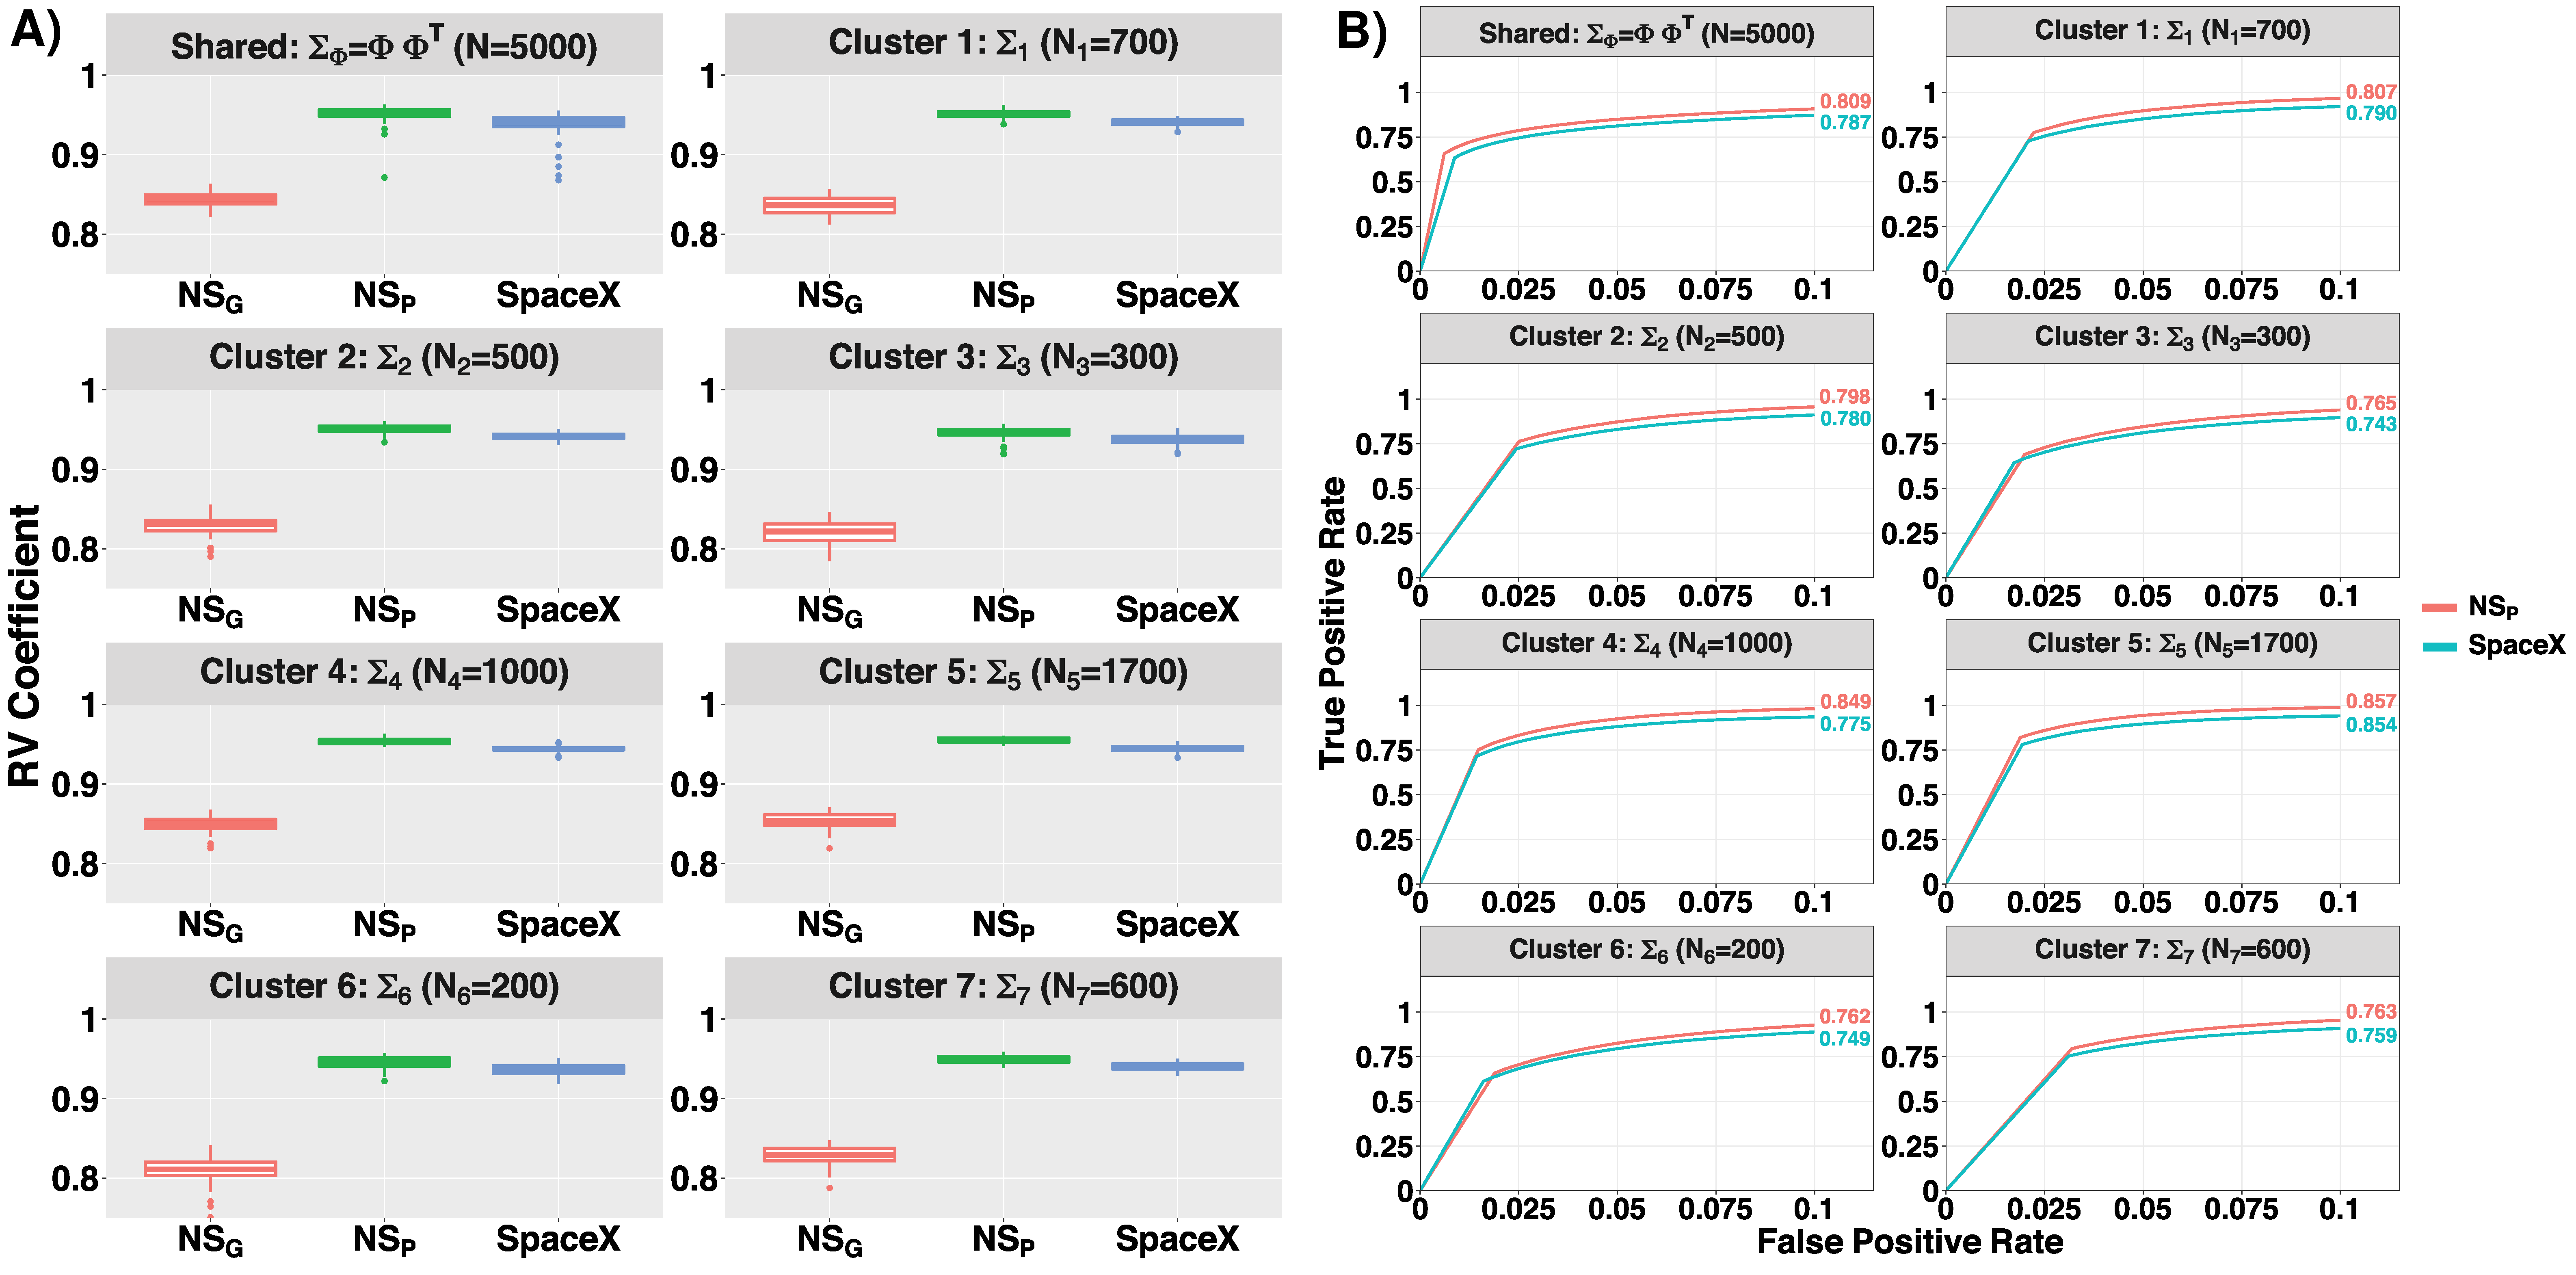
\includegraphics[width=176.18in]{images/Null_sim_RV_ROC} 

}

\caption{ **Accuracy comparison of different methodological settings in estimation and recovery of gene co-expression networks in simulation study while the data is generated without any spatial correlation. A)** The RV coefficient measures the distance between the true and estimated networks. In the left panel, we have boxplot of RV coefficients across $50$ replicates for shared and cluster-specific networks. We compare the RV coefficients for 3 different methods (I) SpaceX, (IV) $\text NS_{\text P}$ ($\rho = 0$) and (V) $\text NS_{\text G}$ (the PMM and spatial informations are not taken under consideration). **B) In the right panel**, we use AUC metric as a measure of network recovery. The Figure represents ROC curves with color-coded AUC values of networks for different settings except for $\text NS_{\text G}$ method.}\label{fig:nullsimulationRVAUC}
\end{figure}

\begin{figure}

{\centering \includegraphics[width=143.36in]{images/Null_sim_norm} 

}

\caption{ **Comparison of different methods based on several norms for estimation of gene co-expression in simulation study while the data is generated without any spatial correlation**. Boxplot of Euclidean, log-Euclidean, root-Euclidean, Riemannian distances (Figure A, B, C and D respectively) across  $50$ replicates for $\Sigma_{\Phi} = \Phi \Phi^{T}$ and $\Sigma_{l}$ $(l = 1, \dots , L)$. We provide the definitions of all the norms in Table \\ref{tab:Normtable} and compare the distances for different methodological settings.}\label{fig:nullsimulationnorm}
\end{figure}

\hypertarget{hub-gene-detection-based-simulation}{%
\section{Hub gene detection based simulation}\label{hub-gene-detection-based-simulation}}

Given the lack of ground truth for real data, we used a simulation study mimicking the real data structure, to evaluate the accuracy of the SpaceX method to recover true hub genes. To this end, we generate the data consisting of \(160\) genes and \(5000\) locations with \(7\) clusters; additional design parameters and details about the simulation settings are provided in Section 3 of the paper. Next, we apply our SpaceX model to the simulated data to estimate the hub genes for each of the \(7\) spatial clusters. We classify the hub gene into two categories: one with more than 40\% connectivity (named ``High'') and another with less than 40\% connectivity (named ``Low''). We choose this cut-off based on degree connectivity we found in the real data example (Section 4). Table B.4 shows the percentage of hub gene recovered for each cluster by setting \(3\) different values of the spatial correlation parameter: \(\rho = 0.2, 0.15\) and \(0.1\) corresponding to low, medium and high levels of spatial correlation. The denominator of recovery rate is the total number of hub genes calculated from the true simulation settings whereas the numerator denotes the estimated number of hub genes obtained from the SpaceX method. From Table B.4, we observe that the percentage hub gene recovery increases with an increase as the level of spatial correlations increase \(\rho\) and size of the cluster. For example, cluster 5 (size = 1700) has the following recovery rates 97.5\% , 95.2\%, 92.3\% for highly connected hub genes corresponding to different level of spatial correlations i.e.~\(\rho = 0.2,0.15\) and \(0.1\) respectively. The recovery rates are 97.5\%, 93.2\%, 90.3\% for cluster 5, 4 and 1 respectively with different cluster sizes (\(N_{5}=1700\), \(N_{4}=1000\), \(N_{1}=700\)). As expected, the recovery rate of the hub genes with higher connectivity is more than in the ones with low connectivity.

\begin{center}\includegraphics[width=1.1\linewidth]{images/Table_6} \end{center}

\hypertarget{realdata}{%
\chapter{Real Data Analysis}\label{realdata}}

We applied the SpaceX method on two spatial transcriptomics datasets which are obtained from the preoptic region of the mouse hypothalamus \citep{Moffitteaau5324} and the human breast cancer dataset \citep{staahl2016visualization}. Here we provide details of preprocessing and exploratory analysis of both datasets in section \ref{exploratory}. We illustrate the detailed application of the community detection algorithm on those two datasets in section \ref{communitydetection}.

\hypertarget{exploratory}{%
\section{Exploratory analysis of the datasets}\label{exploratory}}

\hypertarget{merfish-data}{%
\subsection{Merfish Data}\label{merfish-data}}

The MERFISH dataset is obtained from the preoptic area of the mouse hypothalamus \citep{Moffitteaau5324}. The dataset consists of \(160\) genes and corresponding gene expressions are measured in \(4975\) spatial locations. There are \(7\) pre-determined spatial clusters in the dataset named Astrocyte, Endothelial, Ependymal, Excitatory, Inhibitory, Immature, Mature, and the corresponding sizes are \(724\), \(503\), \(314\), \(1024\), \(1694\), \(168\), \(385\) respectively. The dataset consists of \(2\) more clusters named Microglia, Pericytes with cluster sizes \(90\), \(73\) respectively which are less than \(100\). Those two clusters are removed from the dataset. After removing those two clusters, we have gene expressions from \(4812\) locations corresponding to \(160\) genes. There are no genes with more than \(95\%\) zeros reads. The left panel of Figure \ref{fig:zeroperMF} shows the violin plot of the percentage of zero reads among the genes for each cluster in the MERFISH dataset. The Umap representation of the Merfish data has been provided on the right panel of Figure \ref{fig:zeroperMF}.

\begin{figure}

{\centering \includegraphics[width=0.9\linewidth]{images/Merfish_zero_umap} 

}

\caption{Left panel shows the violin plot of percentage of zero reads among the genes for each cluster w.r.t. Merfish data and the right panel shows the Umap.}\label{fig:zeroperMF}
\end{figure}

\hypertarget{breast-cancer-data}{%
\subsection{Breast Cancer Data}\label{breast-cancer-data}}

The human breast cancer dataset contains expression levels from \(5262\) genes measured at \(250\) locations \citep{staahl2016visualization}. We use the SPARK method with \(5\%\) FDR cut-off on p-values to detect \(290\) spatially expressed genes to carry forward our analysis. The violin plot of the percentage of zero reads among the genes for each spatially contiguous cluster in the Breast cancer dataset is shown in the left panel of Figure \ref{fig:BCperzero}. On the right panel of Figure \ref{fig:BCperzero}, we have provided the Umap.

\begin{figure}

{\centering \includegraphics[width=0.8\linewidth]{images/BC_zero_umap} 

}

\caption{On the left panel, we have violin plot of percentage of zero reads among the genes for each cluster w.r.t. Breast Cancer data and the Umap is shown on the right panel.}\label{fig:BCperzero}
\end{figure}

\hypertarget{communitydetection}{%
\section{Community detection}\label{communitydetection}}

The community detection is a downstream analysis of the shared and cluster-specific networks which are obtained from the SpaceX method. The communities are detected by optimizing modularity over partitions in a network structure \citep{brandes2007modularity}. Figure \ref{fig:comMERFISH} and \ref{fig:comBC} show the detected community modules from shared and cluster-specific co-expression networks for MERFISH and breast cancer data respectively.

\begin{figure}

{\centering \includegraphics[width=0.95\linewidth]{images/merfishCom} 

}

\caption{Shared and cell-type specific community detection for Merfish data}\label{fig:comMERFISH}
\end{figure}

\begin{figure}

{\centering \includegraphics[width=0.8\linewidth]{images/BC_Com} 

}

\caption{Shared and cell-type specific community detection for Breast cancer data}\label{fig:comBC}
\end{figure}

\hypertarget{benchmarking-on-real-spatial-transcriptomics-data}{%
\section{Benchmarking on real spatial transcriptomics data}\label{benchmarking-on-real-spatial-transcriptomics-data}}

In this section, we benchmark our models on two real spatial transcriptomics datasets based on model fitting criteria. To this end, we use information-based criteria -- a standard and well-established technique to compare the model fits between hierarchical Bayesian models \citep{gelman2014understanding}. In this case, we use two information criteria-based metrics to assess our model fitting: (i) Bayesian analogue of AIC \citep{akaike1998information}, defined as the Bayesian information criteria (BIC, \citet{watanabe2013widely}); and (ii) Watanabe-Akaike information criterion (WAIC) \citep{watanabe2010asymptotic}, an improvement on the AIC and a fully Bayesian approach to measure model accuracy computed with log pointwise posterior predictive density and then adding a correction for the effective number of parameters to adjust for over-fitting. These criterion based methods are often used for model selection and specifically for spatial datasets \citep{banerjee2003frailty, banerjee2000geostatistical, lee2009performance}. In both cases, lower (relative) values indicate better model fits.

Table \ref{tab:BICWAIC} shows the BIC and WAIC values for the SpaceX and non-spatial Poisson model for both the mouse hypothalamus and breast cancer data. Based on the criteria based values from the Table \ref{tab:BICWAIC}, we can conclude that the SpaceX model is a better fit to both spatial transcriptomics datasets than the non-spatial Poisson model. For example, there is 64.7\% and 46.6\% of relative gain in accuracy of model fitting of the SpaceX model and non-spatial model w.r.t. BIC and WAIC respectively in case of Merfish data. A similar inference can be drawn for the breast cancer data where the relative gains are 66.4\% and 45.5\% for BIC and WAIC respectively in case of model fitting.

BIC (Merfish)

WAIC (Merfish)

BIC (Breast cancer)

WAIC (Breast cancer)

SpaceX Model

13520

43783

24346

54179

Non-spatial Poisson model

38274

82045

72523

99474

\label{tab:BICWAIC} Criteria based values for application of the SpaceX and non-spatial Poisson model to spatial transcriptomics data i.e.~mouse hypothalamus and Breast cancer data.

\hypertarget{list-of-hub-genes-and-edges}{%
\section{List of hub genes and edges}\label{list-of-hub-genes-and-edges}}

A detailed list of hub genes and top edges for both the datasets can be found at \url{https://github.com/SatwikAch/SpaceX}.

\hypertarget{corroboration-with-tcga-breast-cancer-data}{%
\section{Corroboration with TCGA Breast Cancer Data}\label{corroboration-with-tcga-breast-cancer-data}}

To corroborate some of our findings, we consider the TCGA-based gene expression from 67 breast cancer tissues and 20,000 genes using parallel high-throughput sequencing \citep{wirth2011expression, weinstein2013cancer}. To make a fair ``apples-to-apples'' comparison, we used the same intersecting gene set from the spatial transcriptomics based breast cancer data used in our paper \citep{staahl2016visualization}. We used a network-based algorithm: personalized cancer-specific integrated network estimation (PRECISE, \citet{ha2018personalized}) to obtain gene networks. PRECISE is Bayesian method for gene-network reconstruction for bulk-sequencing data that uses a regression-based approach. The PRECISE method detected \(77\) hub genes out of total \(290\) genes compared to the SpaceX method, which detected \(59\) hub genes -- with \(19\) intersecting hub genes using both methods. The list of all the hub genes detected from each method and intersection hub genes from both method can be found at the webiste mentioned below under the name \textbf{BC\_Hub\_genes\_TCGA.csv} (\url{https://github.com/SatwikAch/SpaceX/tree/main/Hub\%20genes}).

Interestingly, multiple collagens genes (COL16A1, COL6A2, COL5A1) are detected as hub genes by both methods. Collagen biosynthesis can be regulated by cancer cells through mutated genes, transcription factors and signaling pathways \citep{xu2019role}. Understanding of the structural properties and functions of collagen in cancer will lead to anticancer therapy. The LUM gene is associated with collagen genes and effectively regulates estrogen receptors and function properties of breast cancer cells \citep{karamanou2017lumican}. Upregulation in FN1 gene indicates development various types of tumors \citep{sun2020high}. XBP1 can induce cell invasion and metastasis in breast cancer cells by promoting high expression \citep{chen2020emerging}. VIM gene
is used as a biomarker for the early detection of cancer \citep{mohebi2020expression}.

\hypertarget{network-similarity-between-cell-type-specific-networks}{%
\section{Network similarity between cell-type specific networks}\label{network-similarity-between-cell-type-specific-networks}}

We further evaluated the performance of SpaceX to detect similarity between cell-cell interactions. To this end, we used Hamming distance, a well-established similarity measure between two networks, which has been used in several network topology based research studies \citep{tian2005hamming, tian2006multicast, ehounou2020minimizing}. In our case, the Hamming distance is equivalent to the distance between their two co-expression networks, i.e., the number of elements having a similar (or different) values in each of the two networks. A low (high) value in Hamming distance between two networks implies those two networks are more (less) similar to each other.

The mouse hypothalamus data consists of 7 cell-type based clusters among 4812 spatial locations. The SpaceX method provides gene co-expression networks specifically for each cell types. Using the Hamming distance as similarity metric, we measure the network similarity between cell-type specific networks obtained from the Mouse hypthalamaous data analyses in Section 4.1 of the paper. The heatmap of the Hamming distances between cell-type specific networks is shown in Figure \ref{fig:hammDist}. We can observe that the co-expression network of immature cell-type is further apart than other cell type specific network in terms of Hamming distance. We rescale the Hamming distance with maximum value such that the distances are in {[}0,1{]} interval. Specifically, the Hamming distances of immature cell type network with other cell type (Endothelial, Astrocyte, Mature, Inhibitory, Excitatory, Ependymal) networks are 1, 0.73, 0.83, 0.79, 0.82, 0.73 respectively. Based on Figure \ref{fig:hammDist}, network of endothelial cell type is distant from other cell-type based networks except for the immature cell-type. The distance of Astrocyte cell-type netwrok from Ependymal and Excitatory are 0.27 and 0.32 respectively. The neuronal cell type specific networks have lower distance than others which leads to infer a higher level of similarity between cell-type based networks than others. This similarity and disparity based finding aligns with multiple prior works which discuss about hypothalamic cell diversity \citep{chen2017single, mickelsen2020cellular}.

\begin{figure}

{\centering \includegraphics[width=0.6\linewidth]{images/Hamming_distance_Merfish} 

}

\caption{The Figure shows heatmap of Hamming distances between cell-type specific networks.}\label{fig:hammDist}
\end{figure}

\hypertarget{ImplementSpaceX}{%
\chapter{Implementation of SpaceX}\label{ImplementSpaceX}}

SpaceX function extimates shared and cluster specfic gene co-expression networks for spatial transcriptomics data. More details about the SpaceX method can be found in the main manuscript. See below for detailed discussion on installation of SpaceX package, Data inputs and outputs followed by an example.

\hypertarget{installation}{%
\section{Installation}\label{installation}}

The package requires a dependency that is not available on CRAN. Install it with:

\begin{Shaded}
\begin{Highlighting}[]
\NormalTok{remotes}\SpecialCharTok{::}\FunctionTok{install\_github}\NormalTok{(}\StringTok{"rdevito/MSFA"}\NormalTok{)}
\end{Highlighting}
\end{Shaded}

You can install the released version of SpaceX from (\url{https://github.com/SatwikAch/SpaceX}) with:

\begin{Shaded}
\begin{Highlighting}[]
\NormalTok{devtools}\SpecialCharTok{::}\FunctionTok{install\_github}\NormalTok{(}\StringTok{"SatwikAch/SpaceX"}\NormalTok{)}
\FunctionTok{library}\NormalTok{(SpaceX)}
\end{Highlighting}
\end{Shaded}

\hypertarget{data-inputs}{%
\section{Data inputs}\label{data-inputs}}

Please make sure to provide both inputs as dataframe.

The first input is \textbf{Gene\_expression\_mat} which is \(N \times G\) dataframe. Here \(N\) denotes the number of spatial locations and \(G\) denotes number of genes.

The second input is \textbf{Spatial\_locations} is a dataframe which contains spatial coordinates.

The third input is \textbf{Cluster\_annotations}.

The fourth input is \textbf{sPMM}. If TRUE, the code will return the estimates of sigma1\_sq and sigma2\_sq from the spatial Poisson mixed model.

The fifth input is \textbf{Post\_process}. If TRUE, the code will return all the posterior samples, shared and cluster specific co-expressions. Please make sure to request for large enough memory to work with the posterior samples. Default is FALSE and the code will return the posterior samples of \(\Phi\) and \(\Psi^c\) (based on definition in equation 1 of the SpaceX paper) only.

\hypertarget{output}{%
\section{Output}\label{output}}

You will obtain a list of objects as output.

\textbf{Posterior\_samples} contains all the posterior samples.

\textbf{Shared\_network} provides the shared co-expression matrix (transformed correlation matrix of \(G_{s} = \Phi \Phi^{T}\)).

\textbf{Cluster\_network} provides the cluster specific co-expression matrices (transformed correlation matrices of \(G_{c} = \Phi \Phi^{T} + \Psi^{c} {\Psi^{c^{T}}}\)).

\hypertarget{example}{%
\section{Example}\label{example}}

Here we provide an example to run the SpaceX method.

\begin{Shaded}
\begin{Highlighting}[]
\CommentTok{\# Reading the Breast cancer data}

\CommentTok{\# Spatial locations}
\FunctionTok{head}\NormalTok{(BC\_loc)}

\CommentTok{\# Gene expression for data}
\FunctionTok{head}\NormalTok{(BC\_count) }

\CommentTok{\# Data processing}
\NormalTok{G }\OtherTok{\textless{}{-}}\FunctionTok{dim}\NormalTok{(BC\_count)[}\DecValTok{2}\NormalTok{] }\CommentTok{\# number of genes}
\NormalTok{N }\OtherTok{\textless{}{-}}\FunctionTok{dim}\NormalTok{(BC\_count)[}\DecValTok{1}\NormalTok{] }\CommentTok{\# number of locations}
\end{Highlighting}
\end{Shaded}

Next, we'll apply the SpaceX method on the Breast cancer dataset.

\begin{Shaded}
\begin{Highlighting}[]
\CommentTok{\# Application to SpaceX method}
\NormalTok{BC\_fit }\OtherTok{\textless{}{-}} \FunctionTok{SpaceX}\NormalTok{(BC\_count,BC\_loc[,}\DecValTok{1}\SpecialCharTok{:}\DecValTok{2}\NormalTok{],BC\_loc[,}\DecValTok{3}\NormalTok{],}\AttributeTok{sPMM=}\ConstantTok{FALSE}\NormalTok{,}\AttributeTok{Post\_process =} \ConstantTok{TRUE}\NormalTok{)}

\CommentTok{\# Shared\_network :: Shared co{-}expression matrix}
\CommentTok{\# Cluster\_network :: Cluster specific co{-}expression matrices}
\end{Highlighting}
\end{Shaded}


  \bibliography{book.bib,packages.bib}

\end{document}
